\documentclass[11pt,a4paper]{article}

\usepackage[utf8]{inputenc}
\usepackage[T1]{fontenc}
\usepackage[english]{babel}
\usepackage[a4paper,margin=2.4cm]{geometry}

\usepackage{amsmath, amssymb, amsthm}
\usepackage{mathtools}
\usepackage{stmaryrd}
\usepackage{booktabs}
\usepackage{tabularx}
\usepackage{array}
\usepackage{caption}
\usepackage{float}
\usepackage{enumitem}
\usepackage{microtype}
\usepackage{xcolor}
\usepackage{listings}
\usepackage{fancyhdr}
\usepackage{titlesec}
\usepackage{graphicx}
\usepackage{tikz}
\usetikzlibrary{positioning, arrows.meta, fit, backgrounds, calc}
\usepackage[hidelinks]{hyperref}

%  ---  Palette shared with the companion reports  ---
\definecolor{ink}{RGB}{26,30,36}
\definecolor{slate}{RGB}{92,101,112}
\definecolor{mist}{RGB}{233,235,238}
\definecolor{rulegrey}{RGB}{188,194,201}
\definecolor{steel}{RGB}{47,72,102}
\definecolor{steellight}{RGB}{124,146,172}
\definecolor{signal}{RGB}{160,32,45}

\hypersetup{
    colorlinks=true,
    linkcolor=steel,
    citecolor=steel,
    urlcolor=steel,
    pdftitle={The Pass-Through Problem: Multi-Agent Epistemic Planning over Maps the Robots Build},
    pdfauthor={Haniel Ulises},
}

\color{ink}

\setlength{\headheight}{22pt}
\pagestyle{fancy}
\fancyhf{}
\fancyhead[L]{\small\textcolor{slate}{\itshape The Pass-Through Problem}}
\fancyhead[R]{\small\textcolor{slate}{\thepage}}
\renewcommand{\headrulewidth}{0.4pt}
\renewcommand{\headrule}{\hbox to\headwidth{\color{rulegrey}\leaders\hrule height \headrulewidth\hfill}}

\titleformat{\section}{\normalfont\large\bfseries\color{ink}}{\thesection}{0.7em}{}
\titleformat{\subsection}{\normalfont\normalsize\bfseries\color{ink}}{\thesubsection}{0.7em}{}
\titleformat{\paragraph}[runin]{\normalfont\bfseries\color{slate}}{}{0em}{}[.]

\captionsetup{font=small, labelfont={bf,color=slate}, textfont=footnotesize}

\theoremstyle{definition}
\newtheorem{definition}{Definition}
\newtheorem{proposition}{Proposition}

\lstdefinestyle{sys}{
    backgroundcolor=\color{mist},
    basicstyle=\ttfamily\scriptsize\color{ink},
    keywordstyle=\color{steel}\bfseries,
    commentstyle=\color{slate}\itshape,
    stringstyle=\color{slate},
    morecomment=[l]{;},
    morekeywords={:types,:predicates,:objects,:agents,:goal,:init,:event,:action,:action-type,:observability-conditions,:precondition,:effects},
    frame=single,
    rulecolor=\color{rulegrey},
    framesep=5pt,
    xleftmargin=6pt,
    xrightmargin=0pt,
    breaklines=true,
    showstringspaces=false,
    columns=fullflexible,
    captionpos=b,
}
\lstset{style=sys}

%  ---  Notation  ---
\newcommand{\Ag}{\mathcal{A}}
\newcommand{\Mod}{\mathcal{M}}
\newcommand{\Ev}{\mathcal{E}}
\newcommand{\prd}{\otimes}
\newcommand{\Kop}[1]{K_{#1}}
\newcommand{\Dop}[1]{D_{#1}}
\newcommand{\Kw}[1]{\mathit{Kw}_{#1}}
\newcommand{\code}[1]{\texttt{\small #1}}
\newcommand{\bay}[1]{\code{#1}}
\newcommand{\ag}[1]{\mathit{#1}}
\newcommand{\op}{\mathit{open}}
\newcommand{\sem}[1]{\llbracket #1 \rrbracket}

\begin{document}

\begin{titlepage}
\centering
\vspace*{2.4cm}
{\color{rulegrey}\rule{\textwidth}{0.8pt}}\\[0.9cm]
{\LARGE\bfseries The Pass-Through Problem\par}
\vspace{0.5cm}
{\large\color{slate} Multi-Agent Epistemic Planning over Maps the Robots Build,\\
and a Knowledge Precondition Enforced as a Fixed Point\par}
\vspace{0.7cm}
{\color{rulegrey}\rule{\textwidth}{0.8pt}}\\[1.4cm]

{\large Haniel Ulises\par}
\vspace{0.3cm}
{\color{slate} Epistemic Robotics}\\
\vspace{0.15cm}
{\color{slate}\today}

\vfill
{\color{slate}\small
In the preceding demonstrations the occupancy grid and the Kripke model are two
views of one fact, and the epistemic layer never asks where a piece of
knowledge came from. This report builds a problem in which it must. A racking
block crosses a thirty by fifty metre hall; exactly one of three pass-through
bays in it is open. Two scouts read bays from their own SLAM maps, a map
exchange is fused into the receiver's map and applied to the model as a
semi-private announcement, and a carrier may cross only a bay it knows to be
open. That precondition is enforced twice: by the executor against the model,
and by the carrier's route, which is the least fixed point of a reachability
formula whose safe set is itself epistemic.

\vspace{0.6em}
On one branch of the policy the two scouts come to know the open bay only
distributedly, and two exchanges make it the carrier's by elimination. The
carrier then drives through a bay no robot surveyed and of which the exchanges
carried no cell. All three branches were executed to the goal in simulation.
Two further results are negative: a formulation of the exchanges as private
announcements admits a policy that exploits a non-serial relation, and a
published footprint of the AWS shelf model permutes the axes of its mesh.}
\vspace{1.2cm}
\end{titlepage}

\tableofcontents
\newpage

%  ======================================================================
\section{Scope}
\label{sec:scope}

The earlier warehouse reports execute epistemic policies over large floors, and
each states that floor area and epistemic difficulty are independent. The
multi-site report coupled them through the location of a proposition. This
report couples them through the source of knowledge: what an agent knows about
the floor is what its own map, or a map it has been sent, contains.

Three claims are advanced; Section~\ref{sec:notestablished} sets out what
the next iteration takes up from them.

\begin{enumerate}[leftmargin=1.4em, itemsep=2pt]
  \item Sensing outcomes, communication and the knowledge precondition of an
        ontic action were each grounded in occupancy grids built by the robots
        during the run, and the three groundings agreed with the epistemic model
        at every step of every run.
  \item On the third branch of the policy, knowledge held only distributedly
        by two agents was transferred to a third by two map exchanges, none of
        which carried a cell of the bay concerned, and the third agent crossed
        that bay.
  \item The carrier's route is the least fixed point of a formula whose safe
        set is the extension of an epistemic formula, evaluated over the model
        the executor maintains; the route exists exactly when the carrier knows
        of an open bay.
\end{enumerate}

Four bounds are stated at the outset. The floor plan of the building is given
to every robot as common knowledge, and only the interiors of the three bays
are left unknown in it. Localisation is the simulator's odometry, so the maps
are records of observation and not an evaluation of SLAM. The radio is assumed
available throughout. And the executor traverses the policy in order, so the
robots act sequentially.

%  ======================================================================
\section{Preliminaries}
\label{sec:prelim}

The vocabulary is that of the companion reports and is restated only where this
report depends on it.

\begin{definition}[Epistemic model]
Let $\Ag$ be a finite set of agents and $P$ a finite set of atoms. An
\emph{epistemic model} is $\Mod = (W, R, V, W_d)$ with $W$ a finite set of
worlds, $R : \Ag \to 2^{W\times W}$, $V : W \to 2^P$, and
$\emptyset \neq W_d \subseteq W$ the designated worlds. A formula holds at
$\Mod$ when it holds at every designated world, and
$\Mod, w \models \Kop{a}\varphi$ iff $\varphi$ holds at every $v$ with
$(w,v) \in R(a)$.
\end{definition}

\begin{definition}[Distributed knowledge]
For a group $G \subseteq \Ag$,
$\Mod, w \models \Dop{G}\varphi$ iff $\varphi$ holds at every $v$ with
$(w,v) \in \bigcap_{a \in G} R(a)$. The group knows distributedly what it would
know if its members pooled what they know.
\end{definition}

Event models, product update and the three action types of the survey domains
are as defined in \emph{Contamination with a Location}, Section~2. One
consequence is used repeatedly below. In a \emph{semi-private} action the agents
outside the audience relate all events of the action to one another, so they
learn that the action occurred and not which event did; in a \emph{private}
action they relate every event to a $\mathit{nil}$ event with precondition
$\top$, so they continue to consider possible that nothing occurred.

\begin{proposition}[Vacuity]
\label{prop:vacuity}
If $(w,v) \notin R(a)$ for every $v$, then
$\Mod, w \models \Kop{a}\varphi$ for every $\varphi$, including $\bot$.
\end{proposition}

\noindent
Proposition~\ref{prop:vacuity} is immediate from the definition of
satisfaction, and is the whole of the defect of Section~\ref{sec:private}. In
$\mathrm{S5}$ every relation is reflexive and the antecedent never holds;
product update does not preserve seriality in general, and the antecedent can
be reached.

%  ======================================================================
\section{The domain}
\label{sec:domain}

Agents $\Ag = \{\ag{west}, \ag{east}, \ag{carrier}\}$, objects
$T = \{t_1, t_2, t_3\}$ of type \code{tunnel}. The initial model has three
worlds, all designated, with $V(w_k) \ni \op(t_k)$ only, and every relation
total:

\[
  s \models C_{\Ag}\big(\op(t_1) \oplus \op(t_2) \oplus \op(t_3)\big),
  \qquad
  s \models \neg\Kw{i}\,\op(t_k) \quad \text{for every } i \in \Ag,\ k \in \{1,2,3\}.
\]

Three static facts are common knowledge,
\[
  \mathit{covers}(\ag{west}, t_1),\qquad \mathit{covers}(\ag{east}, t_3),\qquad \mathit{hauls}(\ag{carrier}),
\]
and no others of those predicates hold. The bay
$t_2$ opens onto the carrier's own lane and is covered by no agent, so the only
way any agent comes to know it is open is by excluding the other two.

\begin{table}[H]
\centering\small
\caption{The actions of the domain, as event models.}
\label{tab:actions}
\begin{tabularx}{\textwidth}{@{}>{\raggedright}p{2.7cm}>{\raggedright}p{2.6cm}X>{\raggedright\arraybackslash}p{2.9cm}@{}}
\toprule
\textbf{Action} & \textbf{Type} & \textbf{Designated events} & \textbf{Observability} \\
\midrule
$\mathit{survey}(i,t)$ & semi-private sensing
  & $\op(t)$; $\neg\op(t)$, each with $\mathit{covers}(i,t) \wedge \neg\Kw{i}\op(t)$
  & $i$ fully, others partially \\
$\mathit{share\text{-}open}(i,j,t)$ & semi-private announcement
  & $\Kop{i}\op(t)$ & $i,j$ fully, others partially \\
$\mathit{share\text{-}shut}(i,j,t)$ & semi-private announcement
  & $\Kop{i}\neg\op(t)$ & $i,j$ fully, others partially \\
$\mathit{cross}(i,t)$ & public ontic
  & $\mathit{hauls}(i) \wedge \Kop{i}\op(t)$, effect $\mathit{delivered}$
  & everyone fully \\
\bottomrule
\end{tabularx}
\end{table}

The goal is $\mathit{delivered}$. It is ontic, and its epistemic content is
the precondition of $\mathit{cross}$: the goal can only be reached by an agent
that knew. \code{plank} grounds the problem into 16 atoms and 72 ground actions.

%  ======================================================================
\section{The plan}
\label{sec:policy}

Aletheia, through the ePlanSys plan solver under \code{strategy=aostar},
returns the policy of Figure~\ref{fig:policy} at depth five, with three leaves,
after 445 expansions and 647 generations.

\begin{figure}[H]
\centering
\begin{tikzpicture}[
  x=1mm, y=1mm,
  act/.style={draw=ink, fill=mist, rounded corners=2pt, inner sep=3.5pt,
              font=\ttfamily\scriptsize, align=center, minimum height=6mm},
  sen/.style={act, draw=signal, thick},
  ev/.style={->, >=Latex, draw=signal, thick},
  seq/.style={->, >=Latex, draw=slate},
  lab/.style={font=\ttfamily\tiny, text=signal, inner sep=1pt}]
  \node[sen] (a) at (0, 0)    {survey(east, t3)};
  \node[act] (b) at (-42, -16) {share-open(east, carrier, t3)};
  \node[act] (c) at (-42, -28) {cross(carrier, t3)};
  \node[act] (d) at (38, -16)  {share-shut(east, carrier, t3)};
  \node[sen] (e) at (38, -28)  {survey(west, t1)};
  \node[act] (f) at (8, -46)   {share-open(west, carrier, t1)};
  \node[act] (g) at (8, -58)   {cross(carrier, t1)};
  \node[act] (h) at (62, -46)  {share-shut(west, carrier, t1)};
  \node[act] (i) at (62, -58)  {cross(carrier, t2)};
  \draw[ev] (a.south) -- ++(0,-4) -| node[lab, pos=0.25, above] {e-open} (b.north);
  \draw[ev] (a.south) -- ++(0,-4) -| node[lab, pos=0.25, above] {e-shut} (d.north);
  \draw[seq] (b) -- (c);
  \draw[seq] (d) -- (e);
  \draw[ev] (e.south) -- ++(0,-5) -| node[lab, pos=0.25, above] {e-open} (f.north);
  \draw[ev] (e.south) -- ++(0,-5) -| node[lab, pos=0.25, above] {e-shut} (h.north);
  \draw[seq] (f) -- (g);
  \draw[seq] (h) -- (i);
\end{tikzpicture}
\caption{The policy returned: nine nodes, depth five, three leaves. Nodes
outlined in red are sensing actions. The recorded run of
Section~\ref{sec:runs} took the rightmost branch.}
\label{fig:policy}
\end{figure}

\subsection{Distributed knowledge, made individual}

Consider the third leaf. After $\mathit{survey}(\ag{east}, t_3)$ returns
$\neg\op(t_3)$ and $\mathit{survey}(\ag{west}, t_1)$ returns $\neg\op(t_1)$,
each scout has settled its own bay and not the other's, since sensing is
semi-private. Then

\[
  s \models \Dop{\{\ag{west},\ag{east}\}}\,\op(t_2)
  \;\wedge\; \neg\Kop{\ag{west}}\op(t_2)
  \;\wedge\; \neg\Kop{\ag{east}}\op(t_2).
\]

The intersection of the two scouts' relations at the designated world contains
one world, the one at which $t_2$ is open; each relation alone contains two.
The two announcements
\[
  \mathit{share\text{-}shut}(\ag{east}, \ag{carrier}, t_3)
  \quad\text{and}\quad
  \mathit{share\text{-}shut}(\ag{west}, \ag{carrier}, t_1)
\]
restrict the carrier's relation to that world, and
$s \models \Kop{\ag{carrier}}\op(t_2)$. Neither announcement mentions $t_2$.


\begin{table}[H]
\centering\footnotesize
\caption{The model after each action of the third leaf, computed by product
update from the grounded task. Each of the last four columns is the set of bays
open in some world the agent, or the pair, considers possible from the
designated worlds: a singleton is knowledge of which bay is open, and a set
without $t_k$ is knowledge that $t_k$ is shut. World and designated counts
agree with those the epistemic state logged during the recorded run.}
\label{tab:models}
\setlength{\tabcolsep}{4pt}
\begin{tabular}{@{}lrrllll@{}}
\toprule
\textbf{After} & $|W|$ & $|W_d|$ & $\ag{west}$ & $\ag{east}$ & $\ag{carrier}$ & $D_{\{\ag{west},\ag{east}\}}$ \\
\midrule
\code{initial} & 3 & 3 & $\{t_1, t_2, t_3\}$ & $\{t_1, t_2, t_3\}$ & $\{t_1, t_2, t_3\}$ & $\{t_1, t_2, t_3\}$ \\
\code{survey\_east\_t3} $\to$ \code{e-shut} & 3 & 2 & $\{t_1, t_2, t_3\}$ & $\{t_1, t_2\}$ & $\{t_1, t_2, t_3\}$ & $\{t_1, t_2\}$ \\
\code{share-shut\_east\_carrier\_t3} & 3 & 2 & $\{t_1, t_2, t_3\}$ & $\{t_1, t_2\}$ & $\{t_1, t_2\}$ & $\{t_1, t_2\}$ \\
\code{survey\_west\_t1} $\to$ \code{e-shut} & 3 & 1 & $\{t_2, t_3\}$ & $\{t_1, t_2\}$ & $\{t_1, t_2\}$ & $\{t_2\}$ \\
\code{share-shut\_west\_carrier\_t1} & 3 & 1 & $\{t_2, t_3\}$ & $\{t_1, t_2\}$ & $\{t_2\}$ & $\{t_2\}$ \\
\code{cross\_carrier\_t2} & 1 & 1 & $\{t_2\}$ & $\{t_2\}$ & $\{t_2\}$ & $\{t_2\}$ \\
\bottomrule
\end{tabular}
\end{table}

\noindent
The size of the model never changes along this branch: three worlds
throughout, with only the designated set and the relations narrowing, until the
public crossing collapses it to one. The fourth row is the one the domain
exists for: the pair's column is a singleton and neither member's is.

The planner could equally have routed the knowledge through a scout,
\[
  \mathit{share\text{-}shut}(\ag{west}, \ag{east}, t_1)
  \;\text{ followed by }\;
  \mathit{share\text{-}open}(\ag{east}, \ag{carrier}, t_2),
\]
the second an announcement by a speaker who knows $t_2$ is open without having
observed it. That plan has
the same depth. The one returned sends both findings to the carrier directly.

\subsection{The crossing is an announcement}

$\mathit{cross}$ is public, and its precondition contains
$\Kop{\ag{carrier}}\op(t)$. Every agent observes the event and therefore
learns that its precondition held at the actual world. After it the model
contains one world, and $s \models C_{\Ag}\,\op(t_2)$: the scouts learn which
bay was open from seeing the carrier go through.

%  ======================================================================
\section{A private announcement makes the carrier know everything}
\label{sec:private}

The exchanges were first written as private announcements, with the third
agent oblivious. The planner returned a policy of depth four with two leaves,
after 212 expansions; on its second leaf the carrier crosses $t_1$ after being
told only that $t_3$ is shut, and the plan validator accepted it.

The trace of the product updates locates the fault. Let
$\mathit{share\text{-}shut}(\ag{east}, \ag{west}, t_3)$ be executed privately.
The carrier is oblivious to it, and its relation at the designated worlds leads
to the copies produced by the $\mathit{nil}$ event, at which $\ag{west}$ does
not know $\neg\op(t_3)$. Let $\mathit{share\text{-}shut}(\ag{west},
\ag{carrier}, t_3)$ follow, with precondition $\Kop{\ag{west}}\neg\op(t_3)$.
The carrier observes it fully, so its relation is restricted to worlds at which
that precondition holds, and there are none among the worlds it considered
possible. Its relation at the designated worlds is empty, and by
Proposition~\ref{prop:vacuity} $\Kop{\ag{carrier}}\op(t_1)$ holds.

\begin{table}[H]
\centering\footnotesize
\caption{The private variant along its second leaf, in the notation of
Table~\ref{tab:models}. After the second exchange the carrier's relation at
both designated worlds is empty, so the set of bays it considers possible is
empty, and $\Kop{\ag{carrier}}\varphi$ holds for every $\varphi$.}
\label{tab:private}
\setlength{\tabcolsep}{4pt}
\begin{tabular}{@{}lrrllll@{}}
\toprule
\textbf{After} & $|W|$ & $|W_d|$ & $\ag{west}$ & $\ag{east}$ & $\ag{carrier}$ & $D_{\{\ag{west},\ag{east}\}}$ \\
\midrule
\code{initial} & 3 & 3 & $\{t_1, t_2, t_3\}$ & $\{t_1, t_2, t_3\}$ & $\{t_1, t_2, t_3\}$ & $\{t_1, t_2, t_3\}$ \\
\code{survey\_east\_t3} $\to$ \code{e-shut} & 3 & 2 & $\{t_1, t_2, t_3\}$ & $\{t_1, t_2\}$ & $\{t_1, t_2, t_3\}$ & $\{t_1, t_2\}$ \\
\code{share-shut\_east\_west\_t3} & 5 & 2 & $\{t_1, t_2\}$ & $\{t_1, t_2\}$ & $\{t_1, t_2, t_3\}$ & $\{t_1, t_2\}$ \\
\code{share-shut\_west\_carrier\_t3} & 7 & 2 & $\{t_1, t_2\}$ & $\{t_1, t_2\}$ & $\emptyset$ & $\emptyset$ \\
\code{cross\_carrier\_t1} & 2 & 2 & $\{t_1, t_2\}$ & $\emptyset$ & $\emptyset$ & $\emptyset$ \\
\bottomrule
\end{tabular}
\end{table}

Informally: an agent that believed nothing had been said, and is then told
something that could only have been learned from what was said, has no world
left that agrees with what it has heard. A planner searching over the model's
semantics will find that agent and use it. The repair is not a restriction on
the planner. Letting the third agent observe that an exchange took place,
without observing its content, makes the exchanges semi-private, which keeps
every relation an equivalence and the model in $\mathrm{S5}$. The policy of
Figure~\ref{fig:policy} is what the planner returns for that domain.

%  ======================================================================
\section{Knowledge from maps}
\label{sec:maps}

Each robot runs its own \code{slam\_toolbox}, remapped from the absolute topic
\code{/map} to its own namespace. Were the three mappers to publish one map,
every observation would be public, and the semi-private sensing the domain
declares would not describe the system executing it.

A knowledge node per robot keeps two occupancy grids on the geometry of the
floor plan: the robot's own SLAM map, resampled, and its \emph{knowledge map},
the own map fused with every map the robot has been sent.

\begin{definition}[Reading of a region]
\label{def:reading}
Let $G$ be a grid and $B$ a set of cells. With the thresholds of
\code{epistemic\_slam}, $B$ is \emph{blocked} in $G$ if some cell of $B$ is
occupied, \emph{clear} if every cell of $B$ is observed free, and
\emph{undecided} otherwise.
\end{definition}

The quantifier is that of \code{plansys2\_epistemic\_perception}. Occupied
dominates unobserved, since no further observation removes an obstacle, and
unobserved dominates free, since a region is only clear when all of it is. The
region read for a bay is its \emph{corridor}, the interior less the
navigation's inflation of 0.35\,m from each wall. A cell within the inflation
band is used by no route, so whether it has been observed says nothing about
whether the bay can be crossed; including it made a scout's verdict depend on
cells a laser at the mouth sees only at grazing incidence
(Section~\ref{sec:defects}).

\paragraph{Sensing} $\mathit{survey}(i,t)$ drives scout $i$ to a standoff of
1.5\,m from the southern mouth of $t$, faces it into the bay, and reports the
event its \emph{own} map decides: $\op(t)$ if the corridor is clear,
$\neg\op(t)$ if blocked. A verdict counts when three consecutive map updates
agree. If the corridor stays undecided, the scout moves in along the bay's
axis over floor its own map shows free, then backs out and parks two metres
along the block, off the carrier's approach.

\paragraph{Communication} $\mathit{share}(i,j,t)$ fuses $i$'s knowledge map
into $j$'s through \code{epistemic\_slam::fuse}. The reply counts the cells $j$
newly holds over the grid and within each bay. The performer then checks $j$'s
knowledge map against the announcement: after $\mathit{share\text{-}shut}$ the
corridor must be blocked, after $\mathit{share\text{-}open}$ clear. A third
outcome is admitted and logged: the corridor undecided in $j$'s map, which is
the case exactly when $i$ knew by elimination.

\begin{figure}[H]
\centering
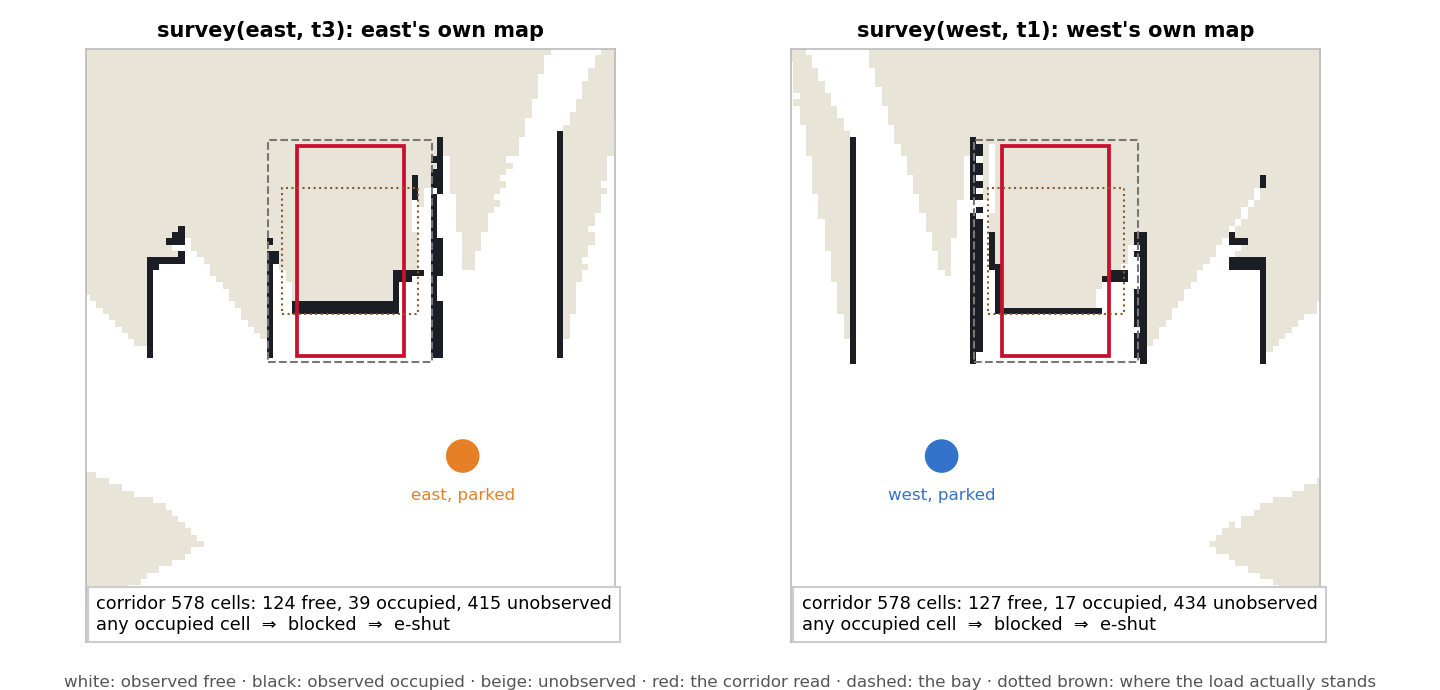
\includegraphics[width=\textwidth]{figures/pass_through_readings.png}
\caption{Each scout's own map at the moment its survey was reported, around the
bay it read, from a second run of the \code{open:=t2} world recorded at every
change of the model. The red box is the corridor. From the standoff most of it
is shadowed by the load; one occupied cell decides \emph{blocked}, and the
load's south face supplies dozens.}
\label{fig:readings}
\end{figure}

\begin{figure}[H]
\centering
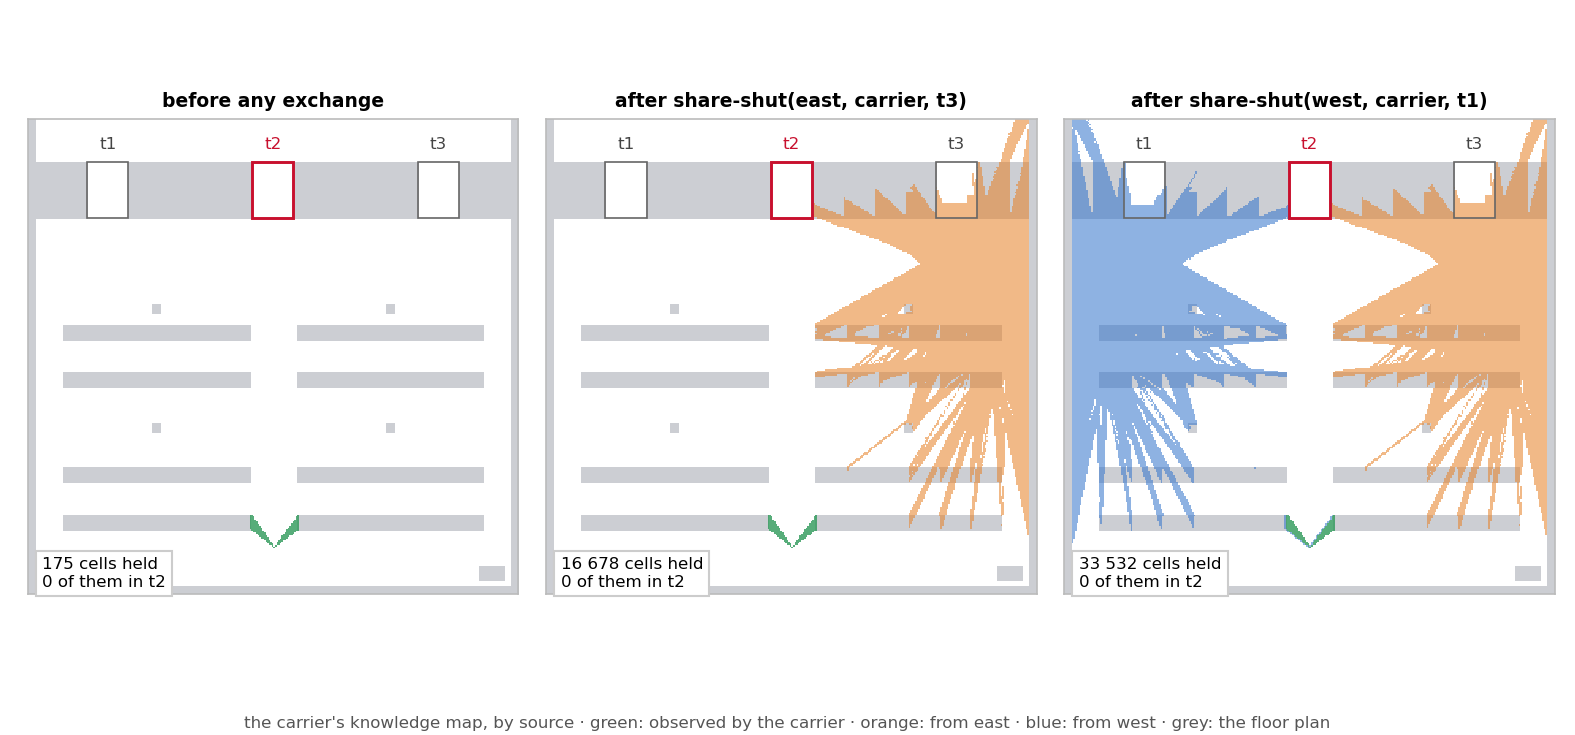
\includegraphics[width=\textwidth]{figures/pass_through_carrier_knowledge.png}
\caption{The carrier's knowledge map before any exchange and after each,
coloured by the robot that observed each cell: 175 cells, then 16\,678, then
33\,532. The corridor of $t_2$ is empty in all three.}
\label{fig:carrierknowledge}
\end{figure}

\paragraph{Soundness of the correspondence} A fusion carries every cell the
sender holds, while an announcement names one bay. The model therefore
under-approximates what an exchange conveys. For preconditions this is the
safe direction: the model never credits an agent with knowledge its map does
not support.

%  ======================================================================
\section{The route is the precondition}
\label{sec:route}

$\mathit{cross}(\ag{carrier}, t)$ drives the carrier along the winning region
of

\[
  W \;=\; \mu Z.\,\big(\mathit{dock} \vee (\mathit{Safe} \wedge \Diamond Z)\big),
  \qquad
  \mathit{Safe} \;=\; \Big\llbracket\, \mathit{free} \;\vee\; \bigvee_{t \in T}
    \big(t \wedge \Kop{\ag{carrier}}\op(t)\big) \Big\rrbracket,
\]

where $\Diamond$ is one step of four-connectivity, $t$ is true at the cells of
bay $t$ in every world, and $\mathit{free}$ reads the floor plan outside the
bays and the carrier's knowledge map inside them. The extension is taken at
every pair of a cell and a world of the model the epistemic state publishes, by
the formula evaluator of \code{mu\_path\_planner}, and restricted to the
designated worlds. Occupied cells are grown by the inflation before the fixed
point is taken.

\begin{proposition}
\label{prop:route}
Let the floor plan be such that no path from the carrier to the dock avoids
every bay, and let no bay be observed occupied in the carrier's knowledge map.
Then the carrier lies in $W$ if and only if, for some bay $t$ traversable in
the plan, either every cell of its corridor is observed free in the carrier's
knowledge map, or $s \models \Kop{\ag{carrier}}\op(t)$.
\end{proposition}

\noindent
The first hypothesis is checked on the floor itself before any file is written
(Section~\ref{sec:floor}). The proposition is the geometric form of the
precondition: a bay the carrier knows open without having seen is safe by the
second disjunct, a bay it has seen free by the first, and a bay it knows
nothing of by neither. The knowledge precondition of $\mathit{cross}$ is
therefore enforced twice and independently: by the executor, which checks
$\Kop{\ag{carrier}}\op(t)$ against the model before dispatching, and by the
route, which does not exist otherwise.

\paragraph{Evaluation} \code{mu\_path\_planner::mu\_reach} computes $W$ by
Kleene iteration, recomputing the backward image of all of $Z_k$ at every step;
on the $310 \times 510$ grid of this floor that is tens of seconds per query.
The package evaluates the same fixed point semi-naively: since the iteration is
monotone, only the cells that entered at step $k$ can admit new cells at step
$k+1$, and propagating from those visits each cell once. The layer at which a
cell enters is the step of the Kleene iteration at which it would have entered,
so the region and the iteration count are the same quantities; a unit test
checks both against \code{mu\_reach} on sixty random floors.

\paragraph{Measured} In the recorded run, before the last exchange $W$ has
51\,428 cells after 327 iterations and stops at the racking; after it,
98\,818 cells after 582 iterations, reaching the carrier through $t_2$, and the
formula lifted $t_2$ and no other bay.

\begin{figure}[H]
\centering
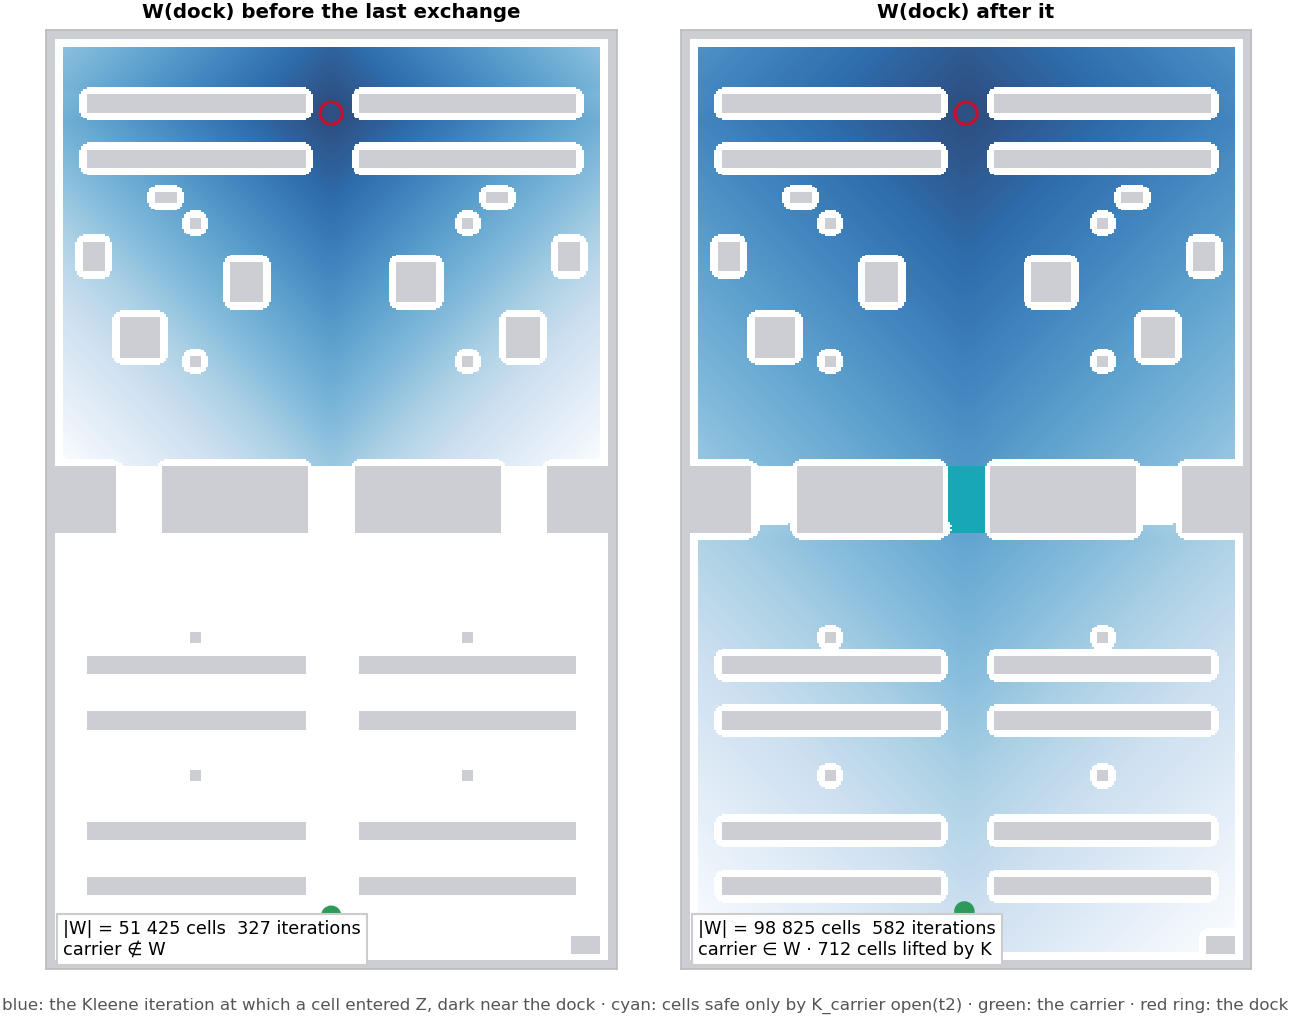
\includegraphics[width=0.86\textwidth]{figures/pass_through_region.png}
\caption{The winning region before and after the last exchange, coloured by the
Kleene iteration at which each cell entered it. Cyan: cells of the bay the
formula lifts. The iteration counts recomputed here from the recorded regions,
327 and 582, equal those the carrier logged.}
\label{fig:region}
\end{figure}

%  ======================================================================
\section{The carrier's own map}
\label{sec:drift}

The carrier maps as it drives, and its own map enters its knowledge map like
any other. Along the lane it is correct at the south end and then slides west:
the rack ends at $x = \pm 1.5$\,m are drawn in place at $y = -18$, 0.3\,m west
at $y = -12$, 0.45\,m at $y = -9$, and by the bay about a metre. A 3.5\,m
scanner in a three-metre lane between repeating racks gives the scan matcher
of \code{slam\_toolbox} little to hold across the lane, and its correction
accumulates there.

\begin{figure}[H]
\centering
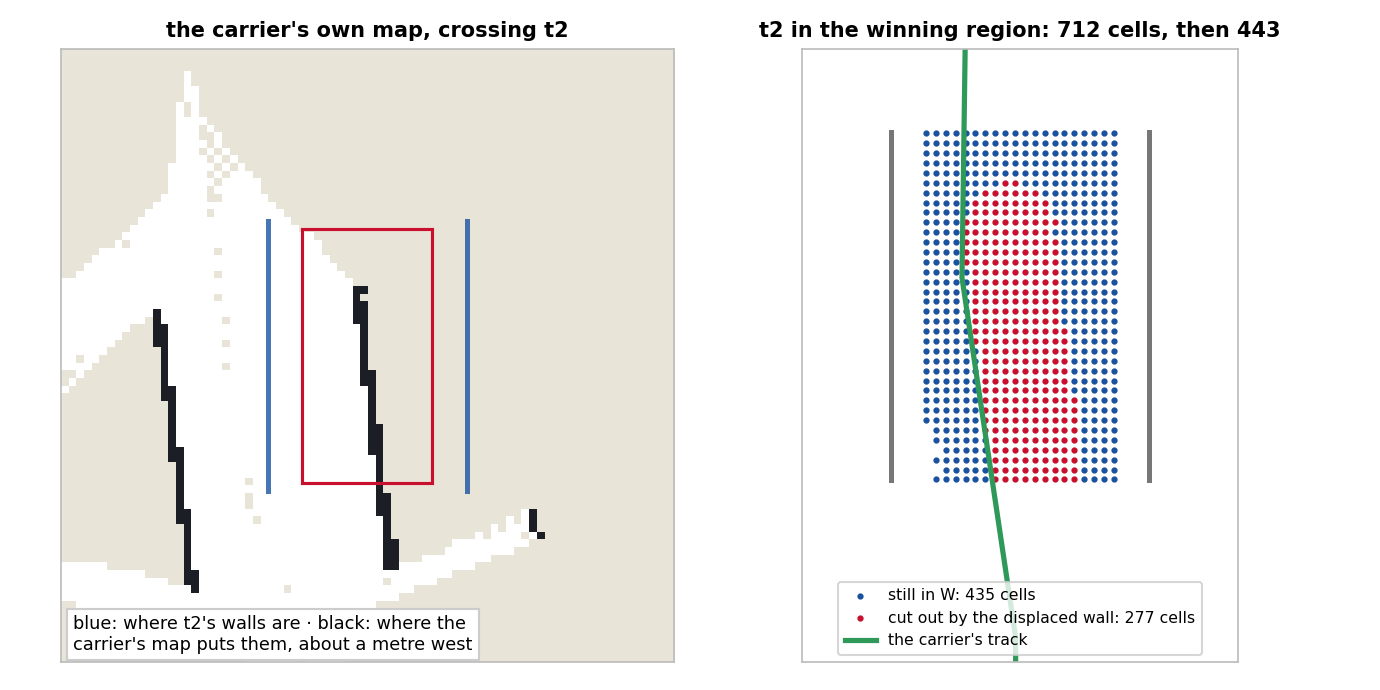
\includegraphics[width=\textwidth]{figures/pass_through_drift.png}
\caption{Left: the carrier's own map while it crosses $t_2$; blue marks where
the bay's walls are, black where the map puts them. Right: the cells of $t_2$
in the winning region before the carrier sees the bay (712) and while it
crosses (435 remain); the displaced wall and its inflation cut out 277, and
the carrier's track runs west of them.}
\label{fig:drift}
\end{figure}

Inside $t_2$ the displaced east wall runs down the middle of the bay, and with
the inflation around it removes a strip from the safe set. The carrier drove
the western strip, at $x \approx -0.5$\,m, and reached the dock. The epistemic
reading is exact. The carrier knew $t_2$ was open by elimination, from two maps
that were right; its own observation of the bay, when it arrived, was wrong,
and the knowledge map merged it without question, since $\mathit{free}$ is read
from that map inside the bays. The route survived because the bay is wider
than the robot, and not because anything reconciled what the carrier had been
told with what it saw.

%  ======================================================================
\section{The floor}
\label{sec:floor}

The hall is the $30 \times 50$\,m \code{OpenRobotics/Warehouse} model; the
racking and the loads are AWS RoboMaker models. The world, the floor plan, the
regions, the robots' poses and the camera shots are written from one layout
file. The block is four rows of shelving from wall to wall with three bays
2.6\,m wide on $x \in \{-10.44, 0, 10.44\}$; the storage and dispatch floors
carry rows either side of a 3\,m lane.

\begin{figure}[H]
\centering
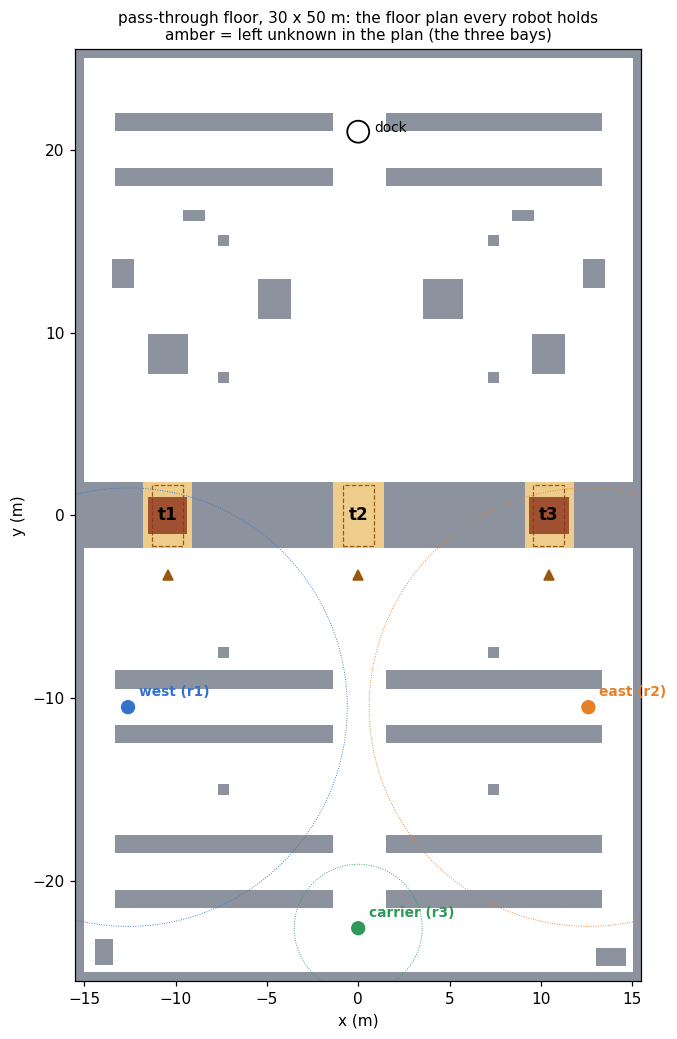
\includegraphics[width=0.55\textwidth]{figures/pass_through_floor.png}
\caption{The floor plan every robot holds. Amber is what it leaves unknown,
the three bays; the loads shown are those of the \code{open:=t2} world and are
in no robot's plan.}
\label{fig:floor}
\end{figure}

Before the plan is written the floor is checked for the properties the mission
depends on: that the carrier cannot reach the dock while no bay is known, that
it can through each bay once that bay is, that a load closes its bay to a robot
with the inflation applied, and that each scout reaches the mouth of its bay
and its parking place. Each placed model's collision mesh is then sliced at
laser height, with its node transform and unit applied, turned and placed as
the world places it, and required to lie inside the box the plan draws for it
to within one cell. The 73 placed models agree to 0.015\,m.

%  ======================================================================
\section{Runs}
\label{sec:runs}

\subsection{The recorded run}

The \code{open:=t2} world was recorded on a $3840 \times 1080$ Xvfb display
with Gazebo on the left half and RViz on the right, and composed into a film of
162\,s whose captions are lines of the run's own log, placed at the instant
they were written. Table~\ref{tab:run} gives the sequence.

\begin{table}[H]
\centering\small
\caption{The recorded run, as the run reported it.}
\label{tab:run}
\begin{tabularx}{\textwidth}{@{}lXl@{}}
\toprule
\textbf{Action} & \textbf{Reported} & \textbf{Model after} \\
\midrule
plan & 9 nodes, 3 leaves, 0.2\,s; carrier $\notin W$ & 3 worlds, 3 designated \\
$\mathit{survey}(\ag{east}, t_3)$ & own map: 168 of 578 corridor cells observed, 37 occupied; $\neg\op$ & 3 worlds, 2 designated \\
$\mathit{share\text{-}shut}(\ag{east}, \ag{carrier}, t_3)$ & 16\,749 cells newly known to the carrier, 163 in $t_3$ & 3 worlds, 2 designated \\
$\mathit{survey}(\ag{west}, t_1)$ & own map: 144 of 578 observed, 17 occupied; $\neg\op$ & 3 worlds, 1 designated \\
$\mathit{share\text{-}shut}(\ag{west}, \ag{carrier}, t_1)$ & 16\,707 cells newly known, 144 in $t_1$, 0 in $t_2$ & 3 worlds, 1 designated \\
$\mathit{cross}(\ag{carrier}, t_2)$ & $t_2$ lifted by $\Kop{\ag{carrier}}$; 43.1\,m; dock after 90\,s & 1 world \\
\bottomrule
\end{tabularx}
\end{table}

\begin{figure}[H]
\centering
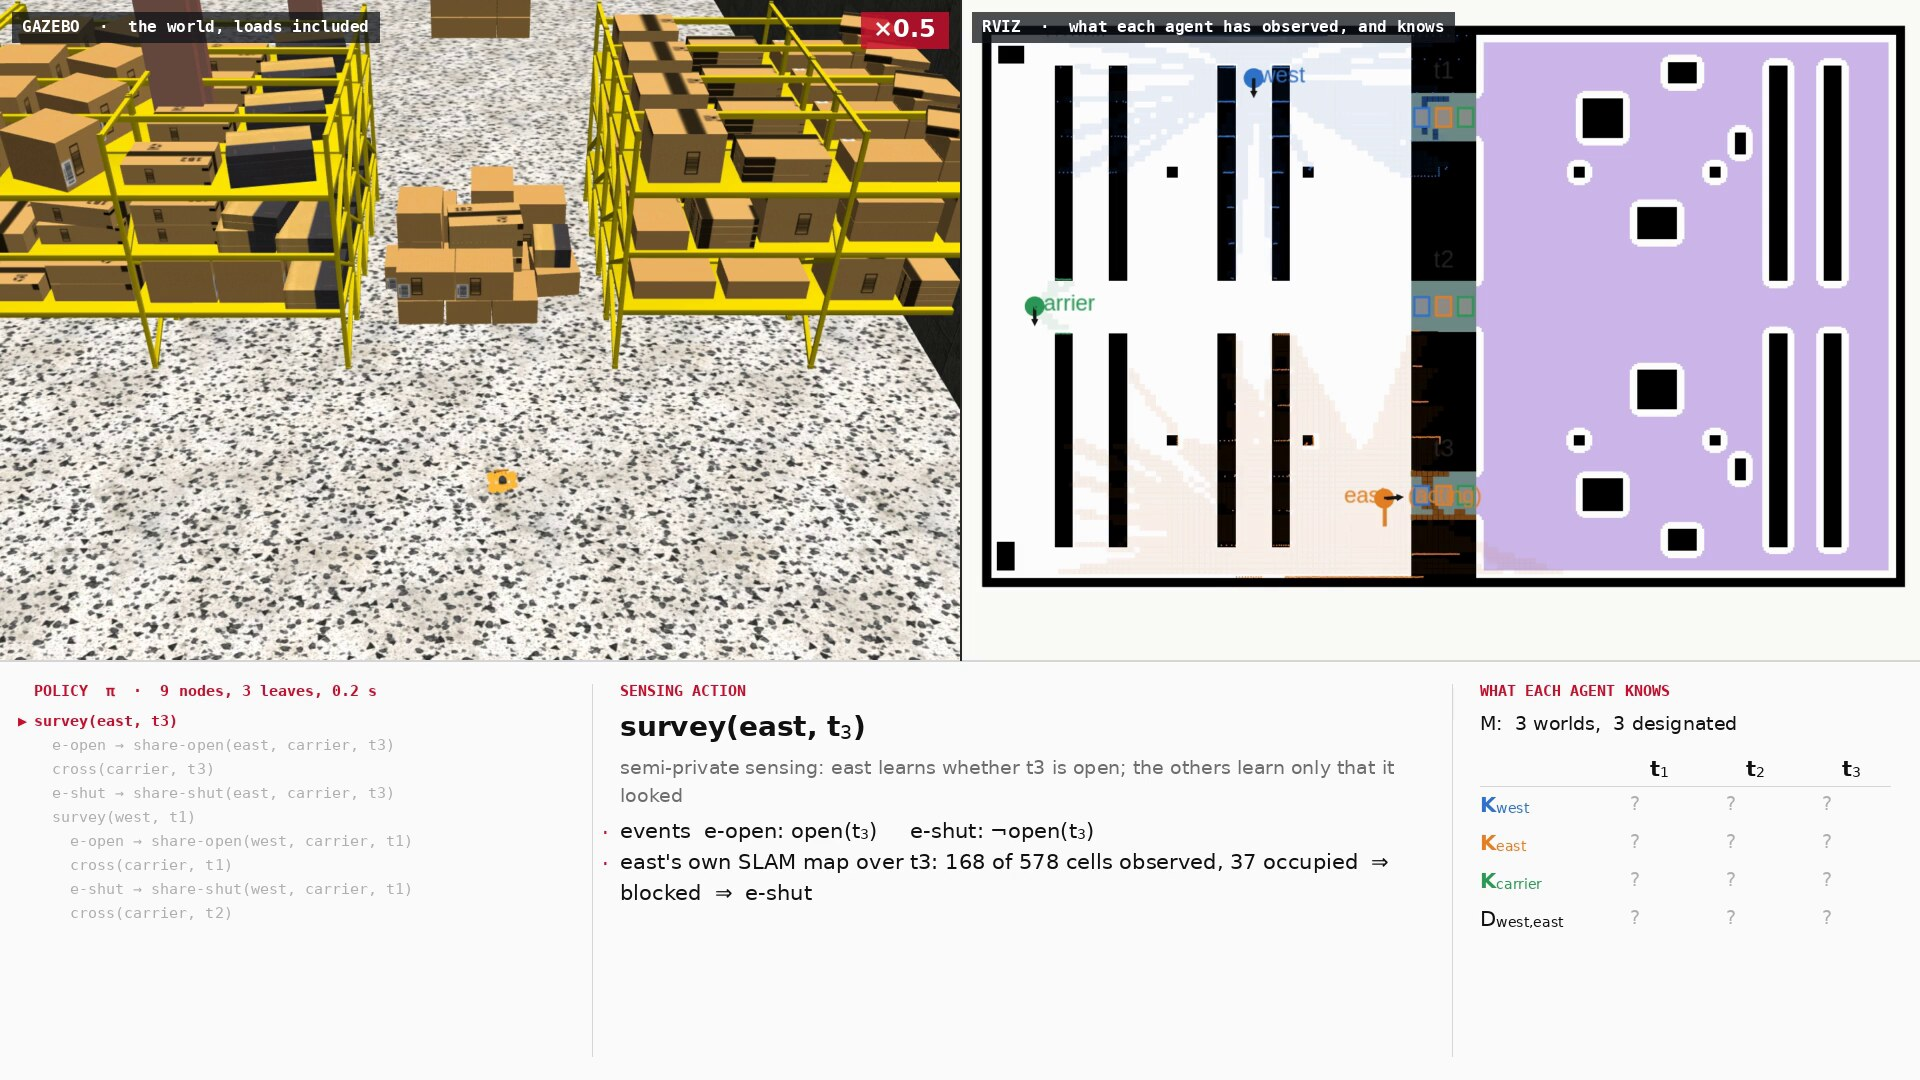
\includegraphics[width=\textwidth]{figures/pass_through_frame_survey.jpg}\\[0.4em]
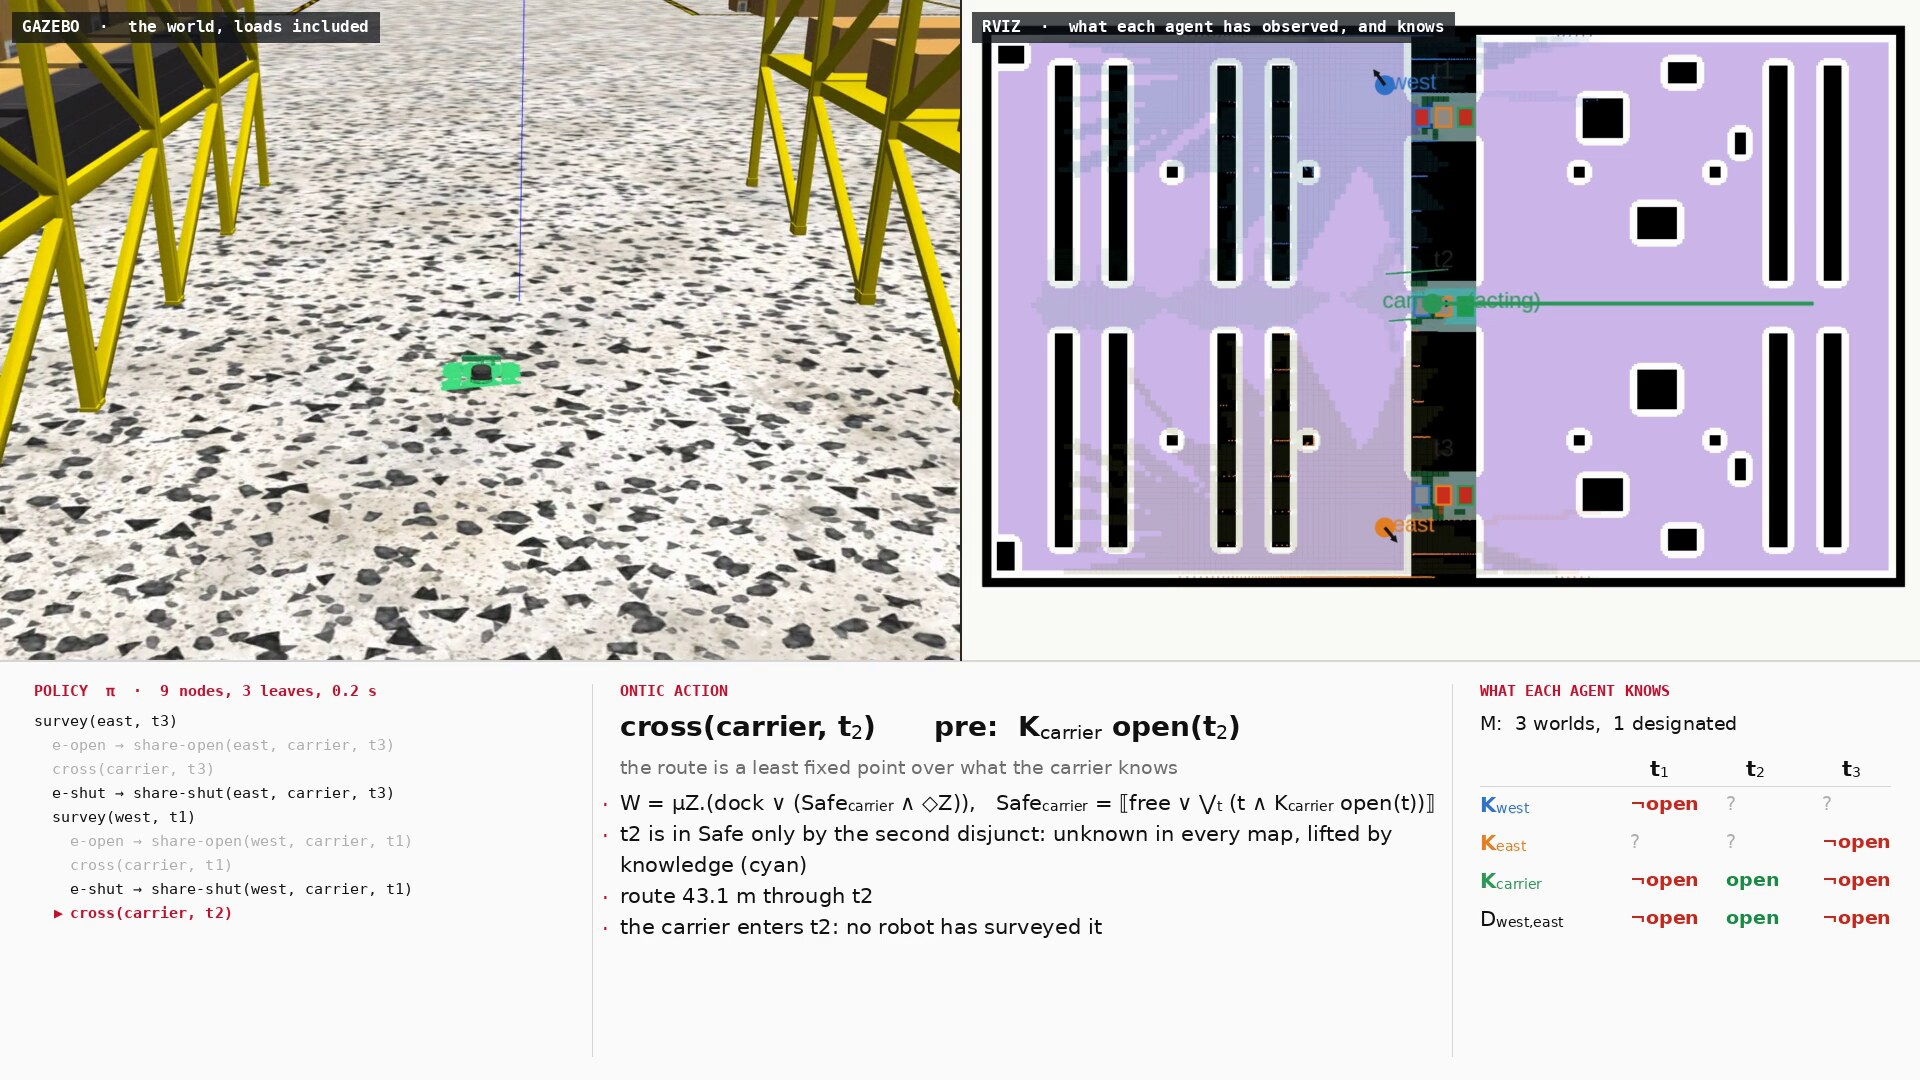
\includegraphics[width=\textwidth]{figures/pass_through_frame_cross.jpg}
\caption{Two frames of the film. Above: $\ag{east}$ at the mouth of $t_3$, with
the load in the bay and the reading of its own map in the panel. Below: the
carrier inside $t_2$; the knowledge table shows $\Kop{\ag{carrier}}\op(t_2)$
beside $\Dop{\{\ag{west},\ag{east}\}}\op(t_2)$, while $\ag{west}$ and
$\ag{east}$ still do not know it individually.}
\label{fig:frames}
\end{figure}

\subsection{Three worlds, three leaves}

The worlds differ by which two bays hold a load and by nothing else. Each was
run headless, and each reached the goal on its own leaf.

\begin{table}[H]
\centering\small
\caption{One policy in three worlds.}
\label{tab:worlds}
\begin{tabular}{@{}llllr@{}}
\toprule
\textbf{Open} & \textbf{Scouts read} & \textbf{Route} & \textbf{Safe by} & \textbf{To dock} \\
\midrule
$t_3$ & $\ag{east}$: $t_3$ clear, 578/578 & 60.6\,m via $t_3$ & observed free & 112\,s \\
$t_1$ & $\ag{east}$: $t_3$ blocked; $\ag{west}$: $t_1$ clear, 578/578 & 60.7\,m via $t_1$ & observed free & 115\,s \\
$t_2$ & $\ag{east}$: $t_3$ blocked; $\ag{west}$: $t_1$ blocked & 43.1\,m via $t_2$ & $\Kop{\ag{carrier}}\op(t_2)$ & 83\,s \\
\bottomrule
\end{tabular}
\end{table}

From the standoff the scouts observed 471 and 453 of an open bay's 578
corridor cells, and in both cases moved in until every cell had been observed.
In the first two worlds the bay crossed is in the carrier's knowledge map,
observed free, and the formula lifts nothing. The third is the only world in
which a robot drives through a bay that no map contains.

%  ======================================================================
\section{Defects}
\label{sec:defects}

\paragraph{The shelves stood a quarter turn from the plan} The footprint of the
AWS ShelfD model was first taken from the table used by the larger warehouse
demonstrations, which gives it as $0.88 \times 2.613 \times 3.918$\,m. Its
collision mesh, read with its node transform and its centimetre unit, is
$3.918 \times 0.88 \times 2.64$\,m: the table permutes the axes. Every unit of
the first floor therefore stood a quarter turn from where its plan put it, the
block was a row of north-south columns with 1.7\,m gaps, and the lasers saw
between them. It was found in the $t_1$ world, where the carrier stopped
0.35\,m short of the south end of a column the plan did not contain. The mesh
check of Section~\ref{sec:floor} rejects that layout and names the same extent.
The table has not been corrected in the package that ships it.

\paragraph{Every cell of a wider region} With a corridor margin of 0.30\,m the
scouts at the mouths of open bays observed 678 and 608 of 714 cells and never
decided. Moving in resolved all but one, in a far corner inside the inflation
band; the corridor of Section~\ref{sec:maps} excludes that band by
construction.

\paragraph{A scout pinned at an aisle end} On the first floor with the corrected
shelves the aisle ends left 1.2\,m to the wall. A scout leaving its aisle there
cut the corner of the row, its laser held it 0.3\,m from the rack, and it did
not move again. The lane was narrowed to widen those gaps to 1.7\,m, shortcuts
are taken against the safe set less one cell, and a robot held by its laser for
two seconds backs off and plans again.

\paragraph{Unknown written as free} The floor plan writes unknown as grey 205,
an occupancy of 0.196. Against a free threshold of 0.25 it reads back as free,
and the three bays arrive open in every robot's plan. The threshold is 0.196,
as map savers write it.

\paragraph{A carrier map that read an open bay as blocked} In the $t_1$ world
and in the recorded run the carrier's own map read the open bay it was
crossing as blocked. Section~\ref{sec:drift} traces it to the drift of that map
along the lane, measured against the rack ends.

\paragraph{A float32 resolution} A grid's resolution crosses a message as a
float32, and a geometry comparison at $10^{-9}$ refused every exchange as not
being on the receiver's grid.

\paragraph{The camera stayed on a shot} Driven at 25 poses per second, the
Gazebo view held two fixed shots and then stayed on the second for the rest of
the run while chase poses were being published. The same switch worked in
isolation. The client renders four or five frames per second under the
software renderer, and a queue of poses is the likeliest reading; it was not
established. At 5\,Hz every cut landed.

%  ======================================================================
\section{What the runs establish}
\label{sec:established}

That a multi-agent epistemic policy can be executed in which every sensing
outcome is decided from the performing agent's own map, every announcement is
carried by a map fusion whose effect on the receiver's map is checked against
the announcement, and the knowledge precondition of the ontic action is
enforced by the reachability of its route as well as by the executor.

That on the branch where it is needed, knowledge held only distributedly by two
agents became individual knowledge of a third through exchanges that carried
none of the cells it concerns, and that the third agent acted on it.

And that one policy reached its goal in each of the three worlds its
uncertainty ranges over.

\section{Directions for the next iteration}
\label{sec:notestablished}

\paragraph{Reconciling what an agent sees with what it was told} The knowledge
map merges every source with one rule, the more confident reading. When the
carrier's own drifted observation of $t_2$ contradicted the bay it knew to be
open, nothing registered the contradiction. A knowledge map that kept its
sources apart, as the epistemic state keeps its worlds, would let the carrier
detect that its own map disagrees with its knowledge, and treat that as
evidence about its localisation.

\paragraph{Localisation from the maps} Poses here are the simulator's odometry,
so the maps are records of observation. With localisation taken from the same
SLAM maps the drift of Section~\ref{sec:drift} would move the robot as well as
the walls, and whether a bay is where the model says it is becomes an
epistemic question in its own right.

\paragraph{Exchanges that carry what the map carries} A fusion carries every
cell the sender holds, while the announcement names one bay. An announcement
generated from the fused cells, one per region the fusion decides, would close
that gap and remove the under-approximation of Section~\ref{sec:maps}.

\paragraph{Communication that can fail} The link is assumed available and the
exchange instantaneous. The link-outage apparatus of \emph{A Link That
Actually Falls} gates exactly the topics an exchange uses, and composing the
two would make the timing of an exchange a planning decision.

\paragraph{A harder epistemic problem} Three worlds and 445 expansions.
More bays, more carriers, or a goal that constrains who else may come to know
would make the search itself the object of measurement.

%  ======================================================================
\section*{Reproduction}

\begin{lstlisting}
ros2 launch pass_through_demo pass_through_launch.py              # open:=t2
ros2 launch pass_through_demo pass_through_launch.py open:=t3
bash tools/validate.sh                                             # no simulator
bash tools/record_demo.sh t2 /tmp/raw.mkv /tmp/run.log             # Xvfb recording
python3 tools/make_video.py --raw /tmp/raw.mkv --log /tmp/run.log \
        --policy /tmp/raw_policy.json --out /tmp/pass_through.mp4
python3 tools/make_floorplan.py --out maps/floorplan \
        --models <aws models>/                                     # floor and mesh checks
\end{lstlisting}

\end{document}
